\subsection{Tasten-Eingabe System}
Natürlich benötigt ein Spiel auch ein sicheres Eingabe-System, welches sowohl die Position der Maus ermittelt, aber auch die Abfrage jeder einzelnen Taste auf der Tastatur regelt. 
Dafür wurde in der FM3D-Engine eine eigene Klasse implementiert, welche sich um dies kümmert.
Um den Nutzer der FM3D-Engine davor zu bewahren nicht jeden einzelnen ASCII-Code jeder Taste auf der Tastatur nachzuschlagen, sind alle Tasten in Form von Makros definiert. 
In dem Namespace FM3D befindet sich die Klasse Inputsystem. Diese Klasse besitzt eine rekursive Instanz, mit welcher man das Inputsystem ansprechen kann. 
Die Klasse beinhaltet außerdem die Enumeration \textit{KEYCLICK}, welches den aktuellen Stand der Maustasten beschreibt. Diese können entweder gedrückt, nicht gedrückt oder losgelassen werden und sind in dieser Enumeration definiert.
Eine Struktur \textit{MOUSE} enthält die Enumeration \textit{KEYCLICK} und einen zweidimensionalen Vektor des Typen \textit{Float}, welcher die zweidimensionale Position im Fenster angibt, an welcher eine Taste der Maus gedrückt wurde.
Diese Struktur wird im Inputsystem als ein vier-Felder Array verwendet, welches jede Taste einer durchschnittlichen Maus beschreibt. Diese sind die linke, die rechte und die mittlere Maustaste. 
Zudem besitzt das \textit{Inputsystem} einen Vektor \textit{lastposinst}, welcher ununterbrochen die Position der Maus ermittelt. Dies ist in den Spielen erforderlich in denen die Maus ununterbrochen die Kamera steuert.

Für die Tastenabfrage wurde zunächst ein Integer Wert verwendet, in welchen der aktuell gedrückte ASCII-Code gespeichert wurde. Dies hat aber den Nachteil, dass nur eine Taste gedrückt sein bzw. abgefragt werden kann. Möchte man nun zum Beispiel einen Spiele-Charakter schräg durch einen Raum durch gedrückte Links- \textbf{und} Rechts-Taste bewegen, so wäre das mit dieser Möglichkeit nicht möglich. Deswegen beschreibt nun ein 121-Felder Array aus booleschen Werten die komplette Tastatur. Jede Feldnummer ist äquivalent zu dem zugeordneten ASCII-Code der Taste. Die Felder [1] bis [4] beschreiben die Maustasten. Einige Felder des Arrays sind nicht von einem ASCII Code auf der Tastatur \textit{belegt} und sind somit "`\textit{frei}"'. Dies hat den Vorteil, dass später simpel weitere Eingabegeräte in das Inputsystem eingebunden werden können.

Die Klasse besitzt Methoden, welche in der Klasse Win32Window.h (Siehe Doxygen Dokumentation), die ein GUI-Fenster abbildet, um die verschiedenen Werte der Arrays und des Vektors zu setzen.
Zudem besitzt die Klasse Methoden, die diese Werte zurück geben. (Für die Verwendung dieser Klasse siehe \cref{inputsystemver})

\begin{figure}
	\begin{center}
		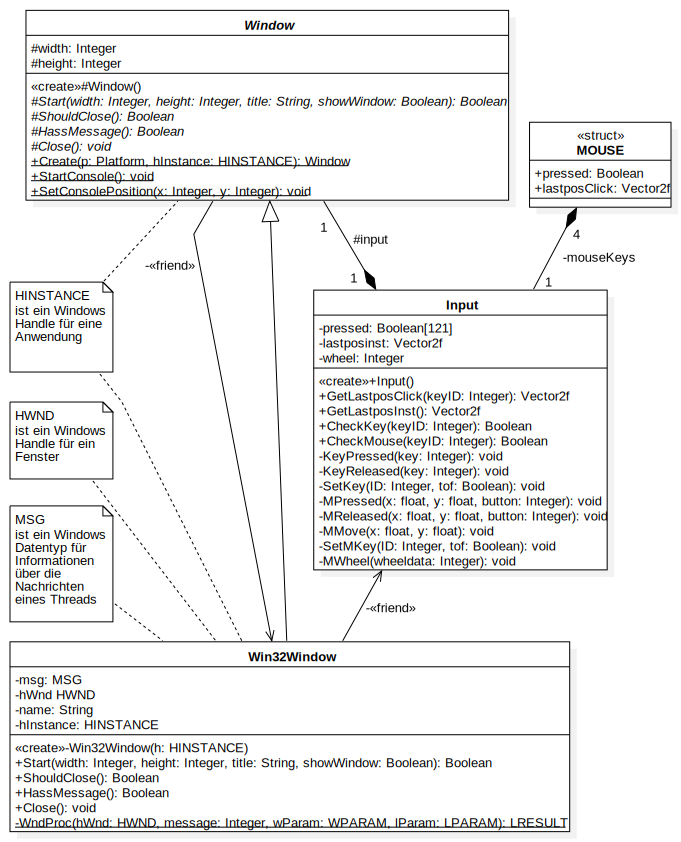
\includegraphics[width=\textwidth]{03unserprogramm/Engine/WindowSystem.pdf}
		Es wurde auf die Angabe von Get- und Set-Methoden sowie Events verzichtet.
		\caption{Window-System}\label{ClassDiagramComponents}
	\end{center}
\end{figure}